\chapter{Cupscanner}\label{chap:cupscanner}

The cup scanning algorithm was designed to take the workspace map (.pgm-file) and the point from which the robot would travel and the point to which it would travel. It returns a list of points where cups have been detected. Figure \ref{fig:cupCollect} illustrates a visualization of the algorithm and together with algorithm \ref{alg:cupscanalgo} a brief overview will be presented here.

\section{Brief overview}
The design of the algorithm had to solve the general problem of how to detect cups from a region determined by the shape of the robot and the two points in which the robot travels between. To solve this problem it is necessary to take into consideration that the robot can travel in any direction, and this can lead to divisions by zero if for instance $arctan$ is used to determine some angle of travelling, thus the algorithm is designed to not utilise mathematical tools which will lead to singularities. The algorithm is designed with help from mathematical vectors to create auxiliary points, and then lines and intersections are calculated with Boost Geometry. Figure \ref{fig:cupCollect} illustrates the geometries which is used to calculate this region of interest, this region is bounded by the bounding box and the red lines. Algorithm \ref{alg:cupscanalgo} explains in more detail what is going on behind the scene. The complexity of the algorithm is $O(N)$, where $N$ is the numbers of points scanned between two points, $N$ is dependent of length of travel and the radius of the robot. As the bounding region that is actually scanned does not match up with the ideal geometry of the robot an error is introduced, this error could possibly lead to cups are not detected or cups are detected without being in the actual range of the robot.

\begin{figure}[htb]
	\centering
	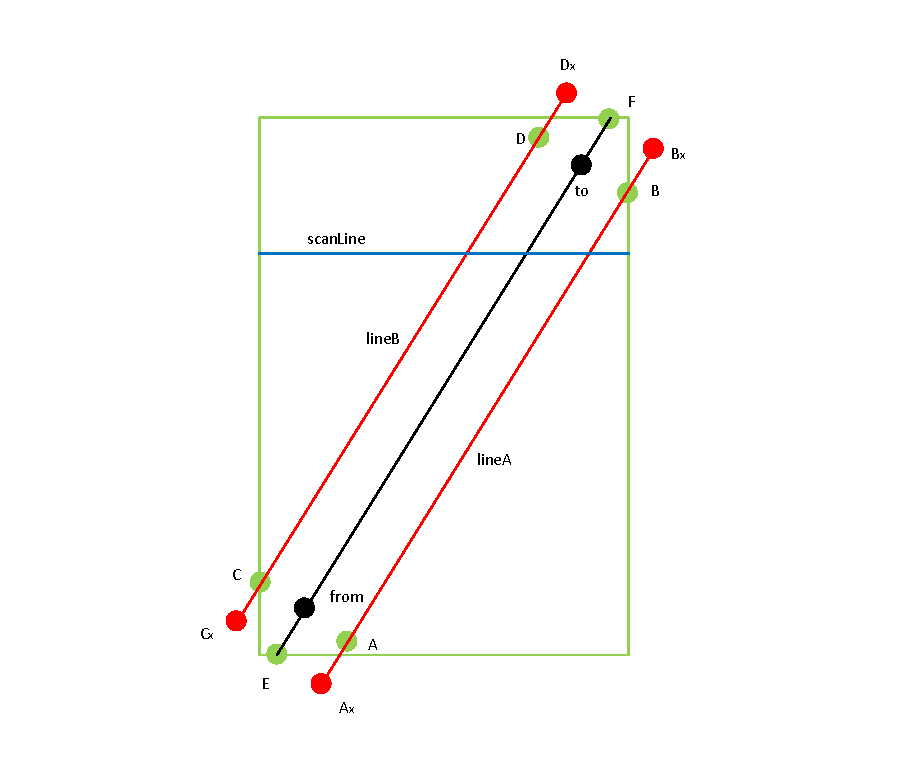
\includegraphics[width=0.8\paperwidth,trim=0 0 0
	0]{graphics/cupCollect.pdf}
	%trim=l b r t (can cut off from every side)
	\caption{Illustrates how the the bounding box (green) and the red lines A and B defines the area of interest.}
	\label{fig:cupCollect}			
\end{figure}

\begin{algorithm}
\caption{Cup scanner algorithm}\label{alg:cupscanalgo}
\begin{algorithmic}[0]
\State \textbf{Input:}
\State $map$\Comment{Workspace map where cups are represented}
\State $from$\Comment{The point where the robot is located}
\State $to$\Comment{The point where the robot needs to go}
\State $radius$\Comment{The radius covered by the robot}
\State \textbf{Output:}
\State $listOfCups$\Comment{A list which contain position of cups detected}
\end{algorithmic}
\begin{algorithmic}[1]
\Function{cupsBetweenPoints}{$map$, $from$, $to$, $radius$}
\State create auxiliary points $A$, $B$, $C$, $D$, $E$, $F$, $A_{x}$, $B_{x}$, $C_{x}$, $D_{x}$ from points $from$, $to$
\State create bounding box $bBox$ from points $A$, $B$, $C$, $D$, $E$, $F$\Comment{Creates area of interest}
\State create auxiliary line $lineA$ from points $A_{x}$, $B_{x}$
\State create auxiliary line $lineB$ from points $C_{x}$, $D_{x}$
\State create auxiliary line $travelLine$ from points $E$, $F$
\For {each $y$ in $bBox$}
	\State clear $listOfIntersections$
	\State create new $scanLine$
	\State set minimum and maximum values of x from $bBox$
	\State calculate intersections between lines $scanLine$, $lineA$, $lineB$, $travelLine$
	\If {number of intersections equals 3}\Comment{Decides if $minX$ and/or $maxX$ needs adjustment}
		\State decide which intersection point has lowest and highest x-value
	\ElsIf {number of intersections equals 2}
		\State decide if intersection with either line $lineA$ or $lineB$ creates a maximum or minimum value of x from the intersection with $travelLine$
	\EndIf
	\For {each $x$ between $minX$ and $maxX$}
		\If {$map(x, y)$ is a cup}
			\State add point to $listOfCups$
		\EndIf
	\EndFor
\EndFor
\State \textbf{return} $listOfCups$
\EndFunction
\end{algorithmic}
\end{algorithm}